\documentclass[../ClassicThesis.tex]{subfiles}
\begin{document}
%************************************************
\chapter{Adjacency Plategraph / Klara}\label{ch:graph}
\newcommand{\TODO}[1]{\textcolor{red}{\\ \textbf{TODO:} #1 \\}}
%************************************************


% Use active Voice (we do….)
% Ein Gedanke pro Paragraph
% Terminologie anpassen über alle Arbeiten hinweg (was ist eine Plate für alle…)
% Jeder sollte eine kleine Related Work section haben
% Erklärungen zu warum dieser Algorithmus genutzt wurde und nicht ein anderer + limitations des gewählten Algorithmus
% Hübsche Bildchen zum anschaulichen Erklären!! (ebenfalls konsistent halten: gleich geformte labels etc.)
% FROM SOLUTION TO PROBLEM /DISCUSSION
% EXPLAIN ALL VARIABLES ETC.!!!

% 1. Was macht es inhaltlich
% 2. Was kann/tut der Graph überhaupt?


% \paragraph{Why is this part necessary?}
On the basis of the graph we can create connectors for plates in a later step ( \ref{ch:joints}). Depending on angles and neighborhood relationships an adequate connector type can be chosen.
% for what? to figure out joint connections?

% \paragraph{What is being achieved in this Chapter?}
In this step we analyse the spatial arrangement of plate objects in 3D-space to create a graph structure which tracks the adjacency. The plates to be analysed are found in the previous step \ref{ch:plates}. Two or more plates are adjacent to another when at least one side touches or overlaps with another plate. In addition, the angles in between the plates are measured. 


% WHAT IS WITH THE 3D SNIPPETS??? DO THEY STILL EXIST?

% \paragraph{Chosen Graph Class Structure}
The graph always holds a list of all found plates and their neighbors. A plate is just one possible object to be listed. Other graph nodes can be left over 3D snippets which will have to be handled when all plates have been correctly connected.\\
For iterating over the graph we traverse all edges of the graph which also hold the important neighborhood parameters such as angle and the line at which nodes intersect.\\\* \\
\hspace*{-1.8cm}
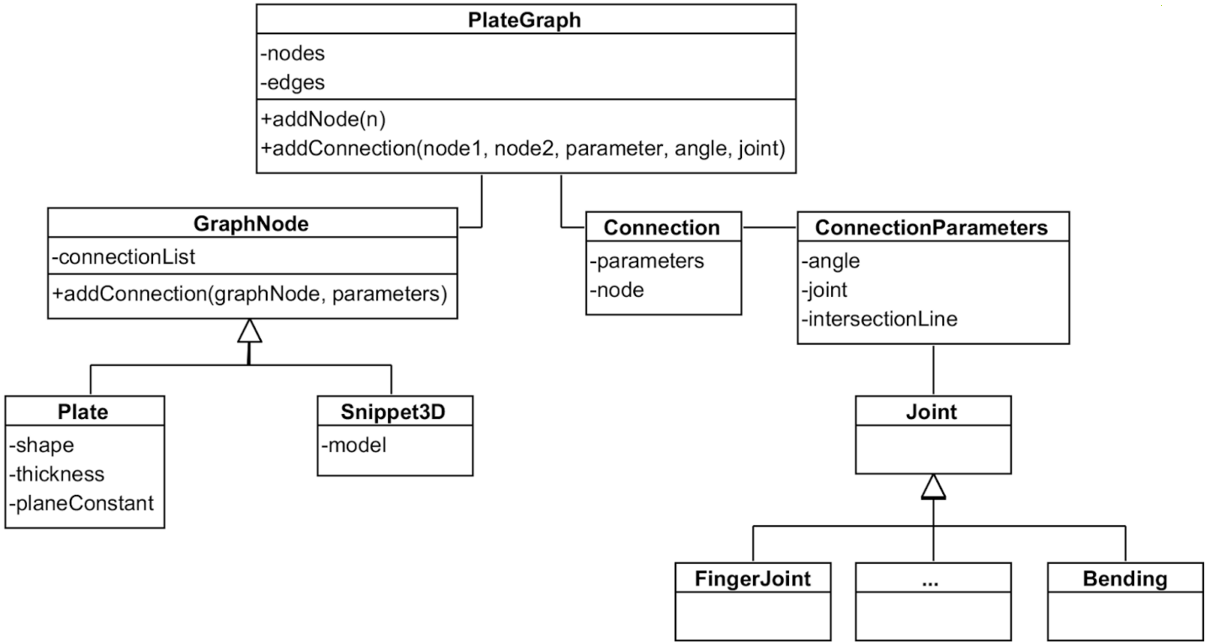
\includegraphics[width=1.3\columnwidth]{Images/GraphStructure.png}


\section{Detecting spatial arrangement}
% \subparagraph{requirements for running the algorithm}
% unnecessary??
As a prerequisite the step \ref{ch:plates} needs to find inherent or create extruded plates first. Afterwards the plane-plane intersections of all combinations of both sides of the plates are computed which results in up to four intersection lines. In preparation for the joint generation step \ref{ch:joints} we truncate the inner intersection lines which would otherwise overlap with adjacent plate intersections.

\subsection{Finding intersections}\label{findIntersections}
% \subparagraph{concrete explanation, functions used/example code etc.}
When two planes intersect there is an intersection line. Since we work with plates which equal 2 parallel planes we expect to find up to 4 intersection lines.\\
Firstly, we retrieve the direction vector(\emph{dir}) of any intersection line between two plates by calculating the cross vector of both normals.
\TODO{include citation}
In order to retrieve all possible intersection lines of two plates we calculate four possible plane-plane intersections \cite{planePlaneIntersection} of 
\begin{itemize}
\item the two main sides of the plates
\item the two parallel sides of the plates
\item one main and one parallel side 
\item and the other way around
\end{itemize}
\*\\
First, a possible position vector has to be found which lies on both planes.
\\\*\\
\emph{Plane constants:} $d_1, d_2$\\
\emph{Normals:} $n_1, n_2$
$$ p = \frac{d_1 * n_{2}^{2} - d_2 * (n_1 * n_2)}{n_{1}^{2} * n_{2}^{2} - (n_1 * n_2)^{2}} * n_1 + \frac{d_2*n_1^2 - d_1*(n_1 * n_2)}{n_1^2 * n_2^2 - (n_1 * n_2)^2} * n_2 $$

On the basis of a position vector and the direction an intersection line can be computed: $ line = p*x + dir$
\\
Now that all lines are found we have to test if the lines actually go through both plates and that the plates touch. \\
In addition, this step retrieves the exact start and end points of the line segment that defines the intersection of both plates.\\
In order to find the boundaries of the lines we calculate the intersections of the lines with all boundary edges of the plates.\\
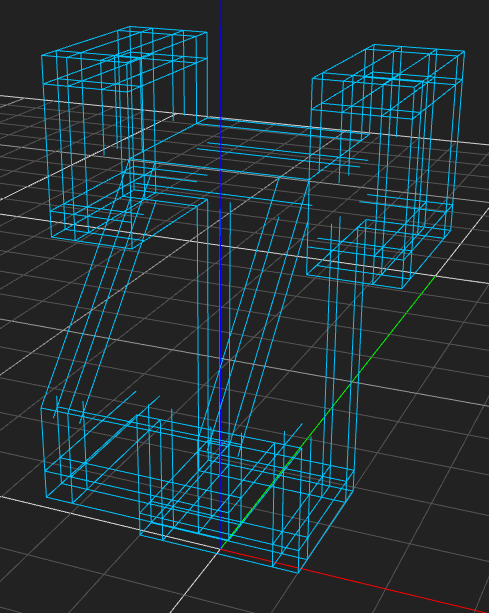
\includegraphics[width=.5\columnwidth]{Images/HeadAllBoundaries.png}
\\
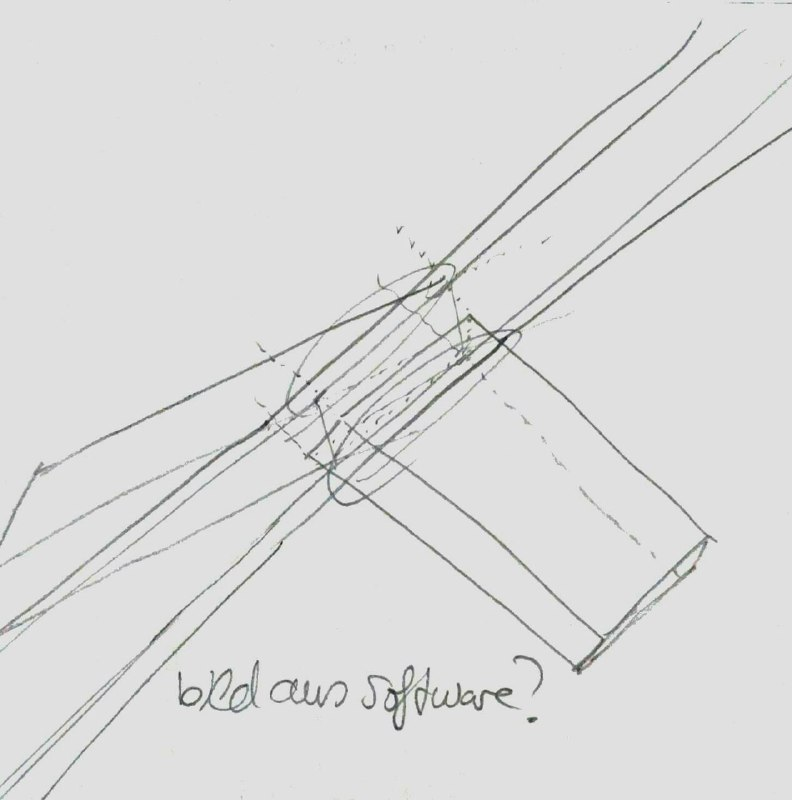
\includegraphics[width=.5\columnwidth]{Images/06-1-graph-fourIntersectionLines.jpg}

\section{Preparing plates for connectors}
\subsection{Volume based clipping}
Before joints can be added to the plates we have to prepare them. We cut the shapes back so that the joints do not overlap with the other plate.\\
As seen before, up to four intersectionlines, have been calculated per intersection.\\
Two of them lie both on one side of the plate and the other two belong to the second side. The two lines on one side build a rectangle when their ends are connected. We use those two rectangles to cut out of the plate what will get fingerjoints.\\
%\textbf{TODO: Insert image of the four lines, with the two rectangles marked.}\\
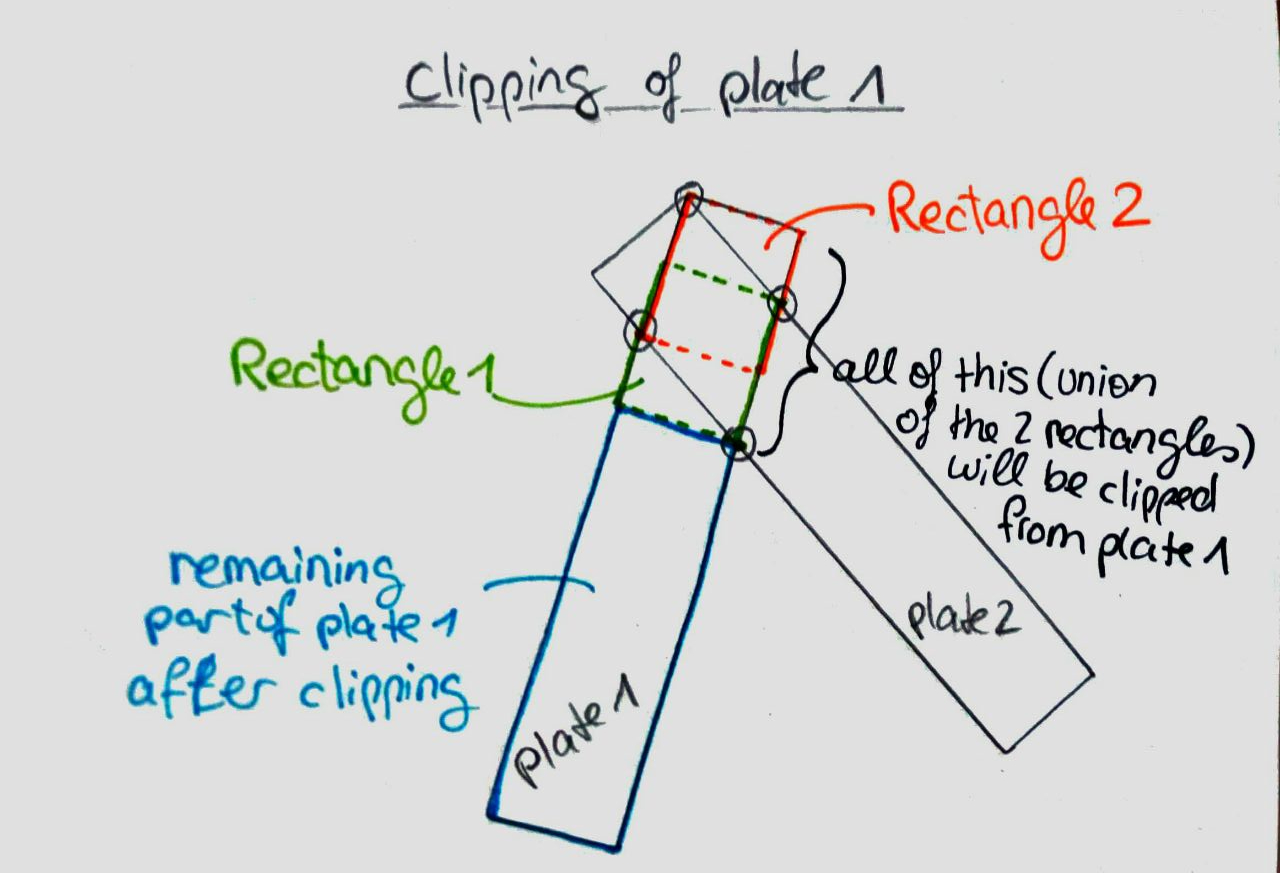
\includegraphics[width=\columnwidth]{Images/10-joints-clippingPlate.jpg}\\
There are cases when not all four lines are actually a plate intersection but only a plane intersection. \\
%\textbf{TODO: Image of plates which result in not 4 intersections.}\\
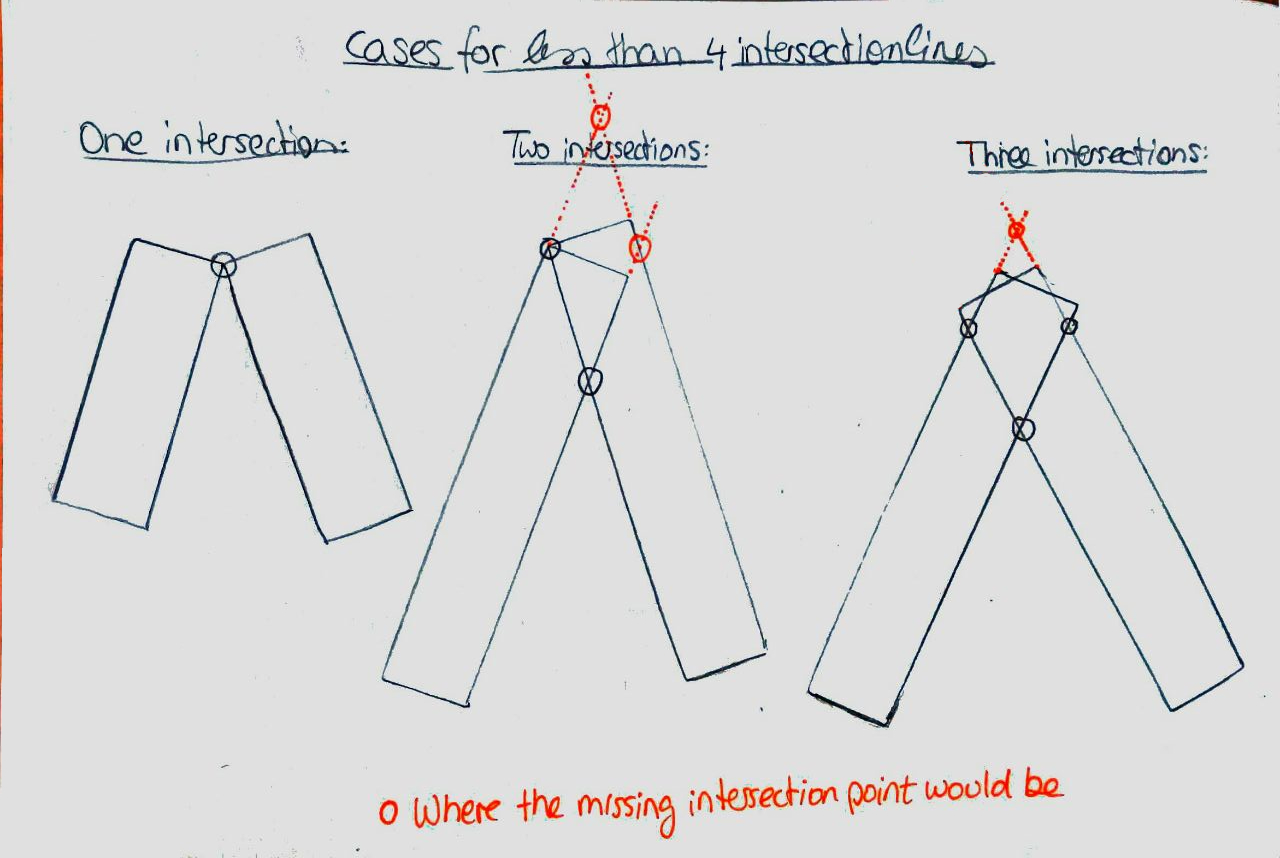
\includegraphics[width=\columnwidth]{Images/10-joints-casesOfLines.jpg}\\
In this case the infinitifly long plane intersection line will be clipped to match the length of the existing plate intersections. This yields two rectangles as well, which can then be used for clipping the shapes of the plates.\\
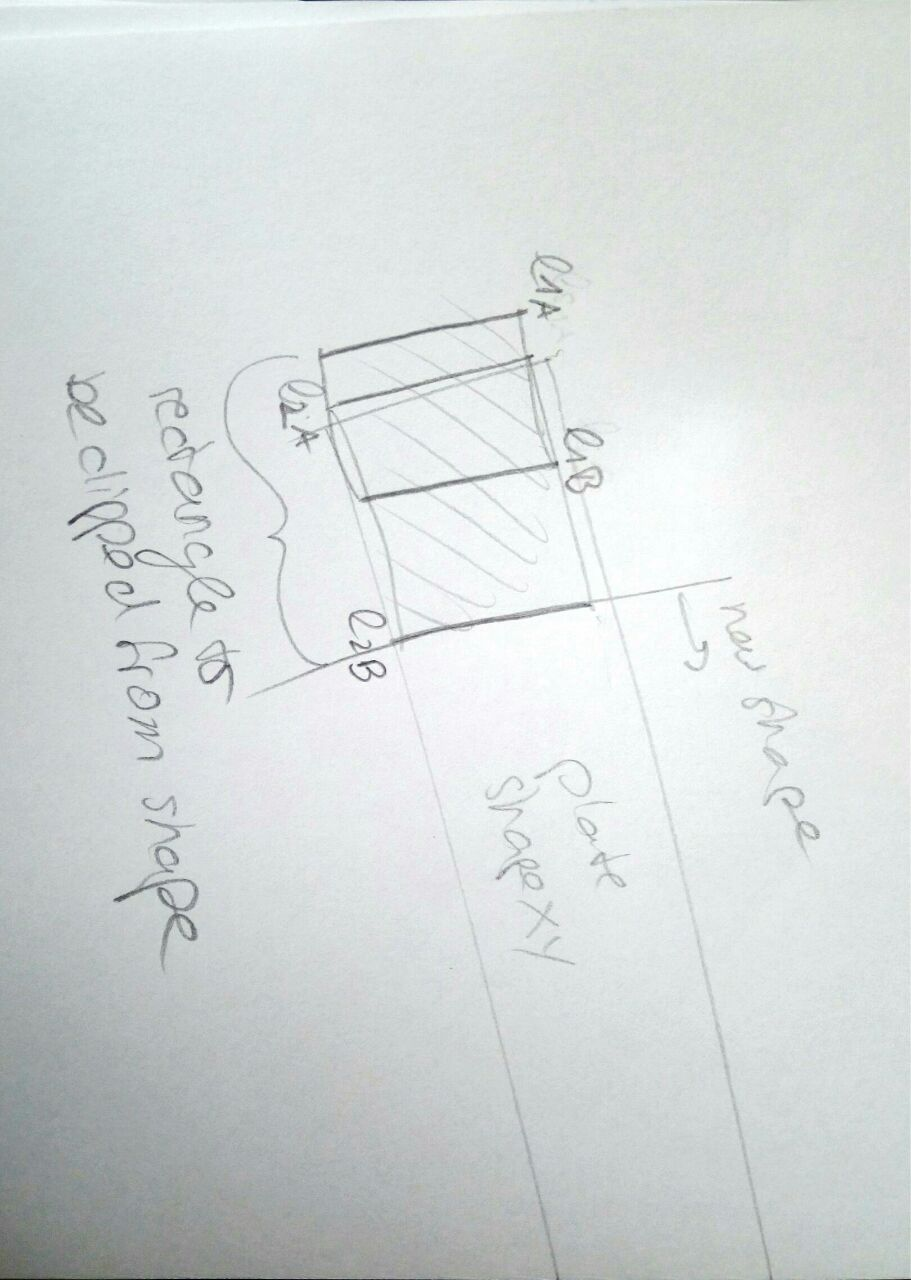
\includegraphics[width=.5\columnwidth, angle=90]{Images/06-1-graph-clippingRectangles.jpg}\\
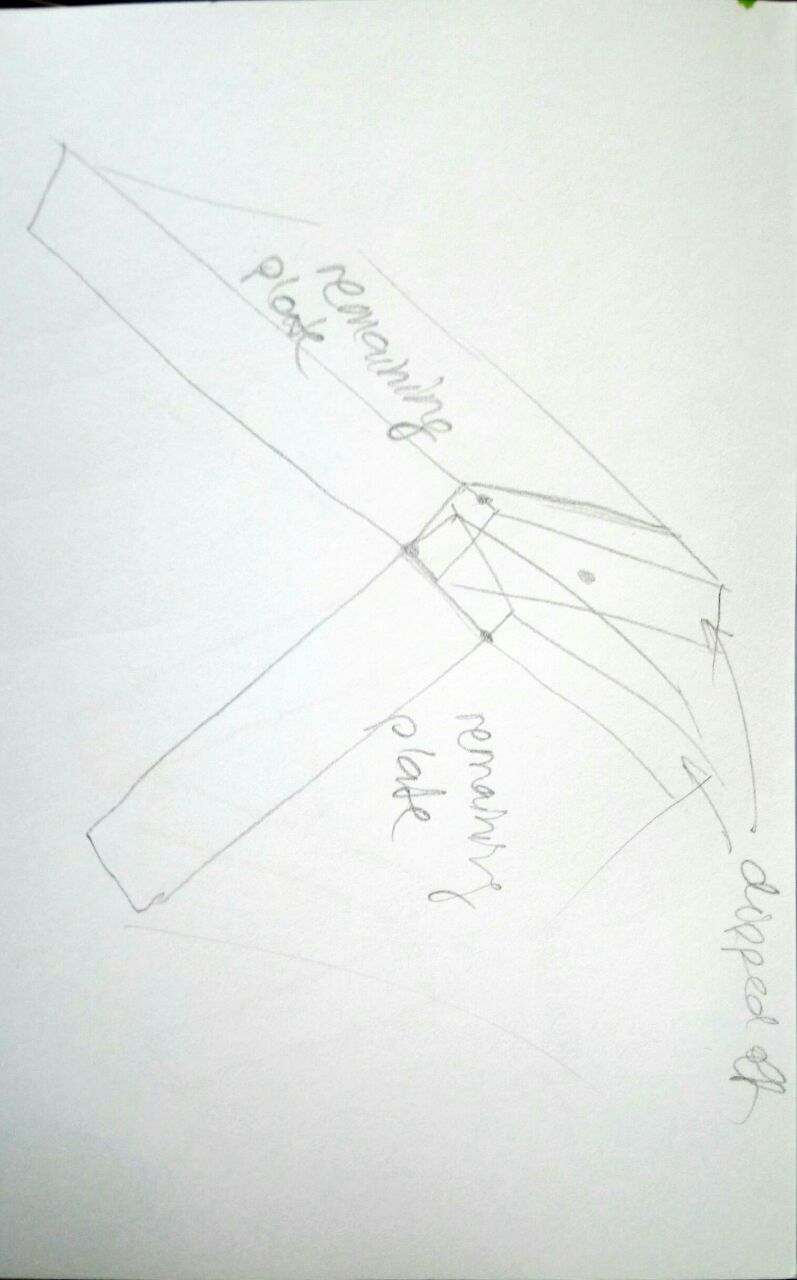
\includegraphics[width=.5\columnwidth, angle = 90]{Images/06-1-graph-clippingResult.jpg}

\section{Analyzing spatial arrangement}
\subsection{Angle calculation}\label{angleCalculation}
In order to generate nicely fitting joints in the upcoming step and for grouping plates to curves (see Chapter \ref{ch:curves}) the angles are necessary.\\
Firstly, we determine the angle between the according planes.\\
plane normals: u, v\\
angle between planes: $\theta$
$$ cos(\theta) = \frac{u \cdot v}{|u| * |v|}$$
But we are not talking about infinitely large planes instead we want the angle which is enclosed by the finitely large plates. Therefore we need to adjust the angle in some cases.\\
Thanks to the previous clipping step we can find out when the angle has to be adjusted.\\
We observed that plates with an acute angle still touch when cut back and that plates with an obtuse angle do not touch after cutting them back.\\
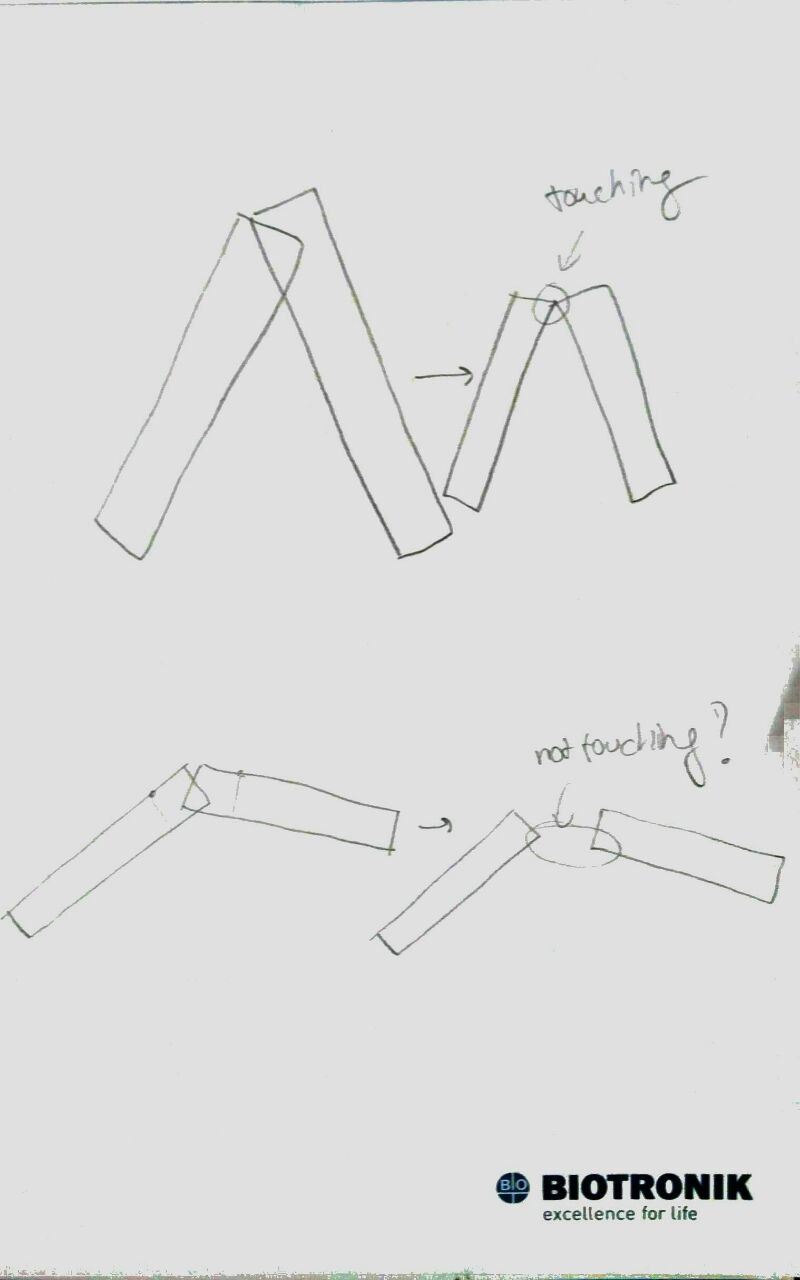
\includegraphics[width=.5\columnwidth]{Images/06-1-graph-TouchingOrNotAfterClipping.jpg}\\
Finally, we test if the plates still touch and adjust the angle accordingly.

\subsection{Finding new main lines}\label{mainLine}
In order to know where to add the joints to the plate we have to identify one line segment for each plate whithin a connection.\\
For that we compare the distances of the new edges of the two plates. Where the distance is the smallest they are the two lines which determine where to place the joints.\\
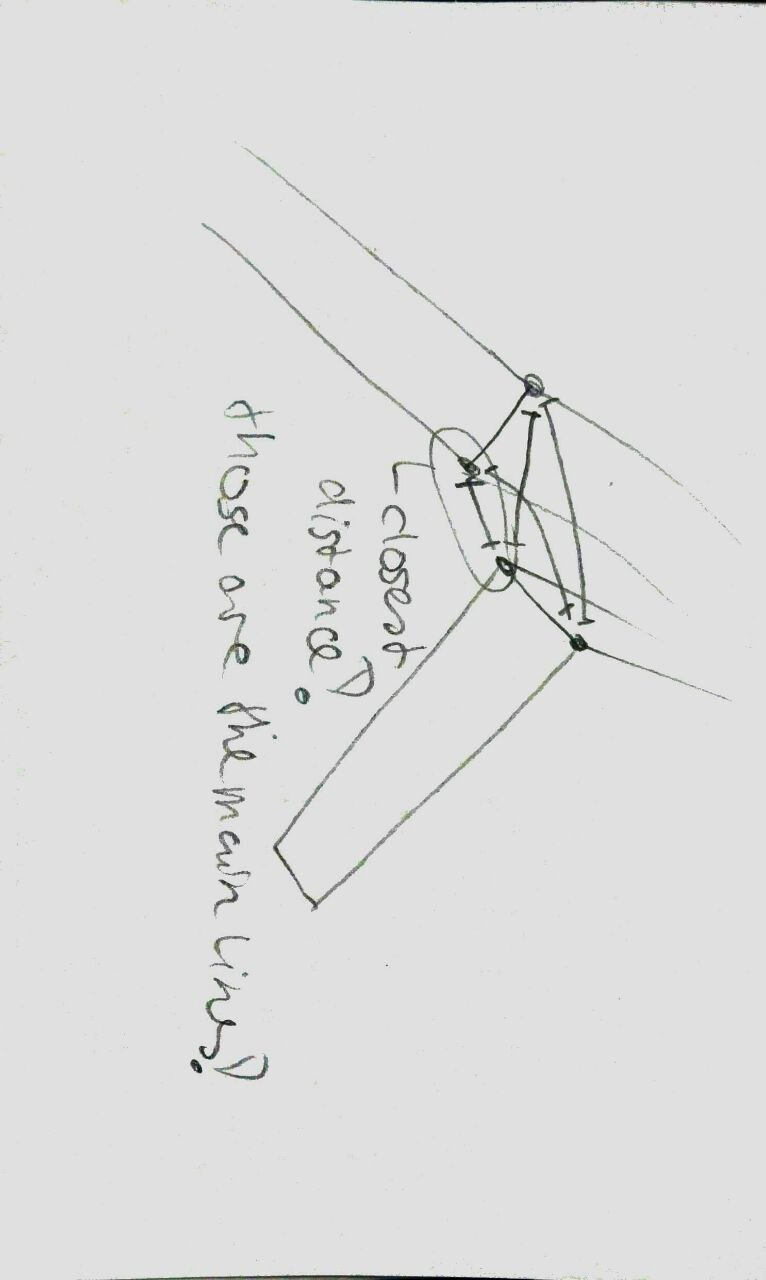
\includegraphics[width=.5\columnwidth, angle=90]{Images/06-1-graph-mainLinesAfterClipping.jpg}\\
The segments are called main line for that connection and plate.

\subsection{Truncating intersection lines}
Now that all main lines are known we need to shorten the lines so that no other lines overlap with it. If this step is missing then the following step for creating joints will run in to problems because the joints overlap each other.\\
If we now have a look at only the inner intersections of plates in a model we can identify the overlaps.
\begin{figure}[t]
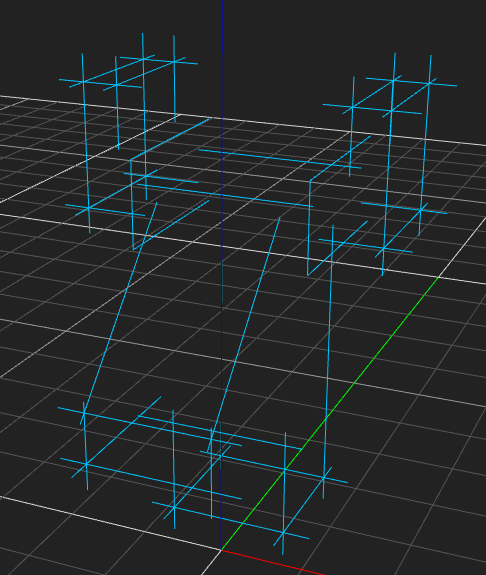
\includegraphics[width=.5\columnwidth]{Images/HeadInnerBoundaries.png}
\caption{The inner boundaries of the plates overlap. In the next step when joints will be created they are only supposed to be on the inner part of the line. Therefore the lines have to be truncated.}
\end{figure}
\*\\
\begin{algorithm}[H]
	\DontPrintSemicolon
	\KwData{lines}
	\KwResult{truncated lines}
	initialize variables here\;
    \For{line$\_$pair in lines}{
    	line1 = line$\_$pair[0]\;
        line2 = line$\_$pair[1]\;
        point = lineLineIntersection(line1, line2)\;
        \If{isPointOnLine(point, line1) and isPointOnLine(point, line2)}
        {
       		\tcp{linesegments actually cross}
       		startSegmentLine1 = new Line(point, line1.start)\;
            endSegmentLine1 = new Line(point, line1.end)\;
            startSegmentLine2 = new Line(point, line2.start)\;
            endSegmentLine2 = new Line(point, line2.end)\;
            \tcp{the shorter part of each line is discarded}
			\eIf{startSegmentLine1.distance() $>$ endSegmentLine1.distance()}{
				\eIf{startSegmentLine2.distance() $>$ endSegmentLine2.distance()}{
				return \{
                    	endSegmentLine1\;
                        endSegmentLine2
                    \}
				}{
                    return \{
                    	endSegmentLine1\;
                        startSegmentLine2
                    \}
				}
			}{
			return \{
                	startSegmentLine1\;
                    startSegmentLine2
                \}
			}	      
        }
    }
   	\caption{Truncate lines}
\end{algorithm}

Finally, we found all plate adjacencies and necessary information on the connected parts. Also, we adjusted the plates. Therefore the next chapter \ref{ch:joints} can start adding joints.

\section{Alternative approaches for problems addressed in this chapter}
The solutions presented in this chapter may not be the only way to go. Therefore, we want to give an overview of other algorithms we tried and why we replaced them.
\TODO{nice introduction for this section and headlines}

\subsection{Finding main lines by checking if they lie on a corner of the shape}
As already mentioned when plates intersect there can be up to four intersection lines. We need to define which of them is the most important one in order to know where to put joints. The line we wanted to choose had to touch both plates.
\TODO{Image of the four lines and showing which one should always be the main line}
This means all lines which intersected with any points of the shapes of the plates were ignored. The other line became main line.\\
Our assumption, which we adopted from the Platener thesis \TODO{cite},  for finding the main line was the following:\\
Two plates always touch one another edge-to-edge. Therefore, if an intersection line does not lie on an outer boundary of the shape then it is the main line.\\
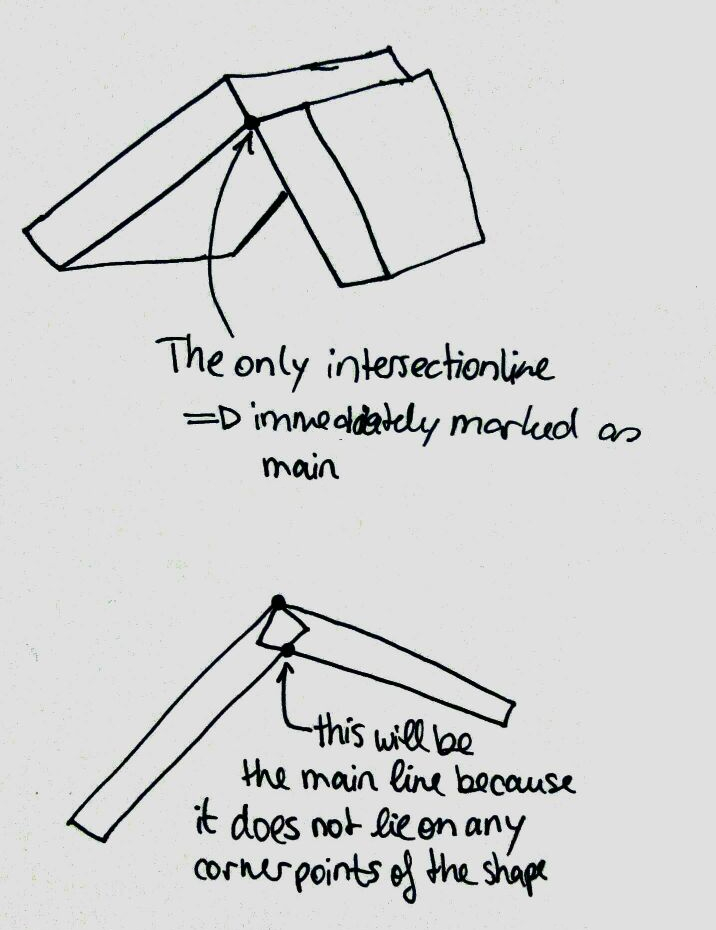
\includegraphics[width=.5\columnwidth]{Images/06-1-graph-assumptionMainLine.jpg}\\
But the problem is that plates can intersect each other in many different ways which do not all verify our first assumption. 
\TODO{include image of two planes where this doesnt work}
This is why we replaced this algorithm with the one from the previous section \ref{mainLine}

\subsection{How we found angles before:}
Our previous version of finding a main line was supposed to yield one line. Based on this line the angle was calculated with the following procedure: 
\TODO{Include image that shows when this is not the case, with captions explaining why our current algorithm fails here}
Therefore, it happens that the current algorithm finds more than one main line. \\
A new approach we developed for that is clipping the plates at all four intersection lines. Based on the result the angle can be determined because the previous angle calculation cannot be used anymore because the main line is not given anymore. \\
\*\\
In order to generate nicely fitting joints in the following step and for grouping plates the angles are necessary.\\
Firstly, we determine the angle between the according planes.\\
plane normals: u, v\\
angle between planes: $\theta$
$$ cos(\theta) = \frac{u \cdot v}{|u| * |v|}$$
But we are not talking about infinitely large planes instead we want the angle which is enclosed by the finitely large plates. Therefore we need to adjust the angle in some cases dependent on the direction in which the normals are pointing. We know which sides of the plates are enclosing the angle thanks to the previous main line calculation.
% figure which shows when angle is right, but also one case when it is not right
\begin{figure}[h]

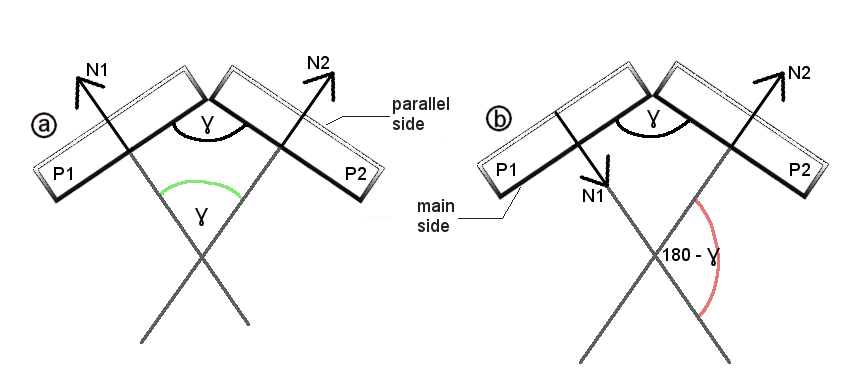
\includegraphics[width= 1\columnwidth]{Images/anglesExamplesSmall.png}
\caption{(a) The angle between the plates' normals correspond with the angle $\gamma$ between the plates. (b) The angle between the plates' normals is in this case an adjacent angle to the requested angle $\gamma$.}
\end{figure}

In order to find out in which cases the angle has to be adjusted we check for two properties.\\
Firstly, there is the question which of the sides of the plates intersect. A plate is defined by a 2D-shape which is called main side. The other side which exists due to a specified thickness of the plate is called parallel side.\\
Additionally, we look at the direction of the normals. The direction is positive when it is directed from the main to the parallel side and negative otherwise.\\
For an angle to be in need to be adjusted the following conditions need to be satisfied.
\begin{itemize}
    \item The two plates touch with the same type of side 
    \item[] AND
    \item Their directions are both positive OR both negative
\end{itemize}


\subsection{Dustin: how he did it}
\TODO{Maybe include this somewhere else....}
Dustin used an adjacency matrix for keeping track of neighboring plates. All the plates were kept in a plate array. Their indices corresponded to the rows and columns of the matrix. Each cell contained a set of plate adjacency objects. This made it possible that one plate could have more than one connection.\\
Furthermore, in the master thesis on Platener a connection is calculated by finding all four possible connections between both sides of two plates. Then the edges of the plates are tested against the line. Those edges, which lied on the line were then tested for overlaps.\\
\*\\
Instead of an adjacency matrix we used the previously explained plate graph class structure because it allows for traversal along the plates and, additionally, the found edges. \\
Moreover, our structure is open for adding additional objects beside plates. For example 3D-printable snippets which cannot be converted to plates by our Software.\\
When looking for plate intersections we also calculate all possible intersections. But plates do not always touch each others edges. Therefore we replaced this algorithm by a different approach explained in \ref{findIntersections}

% \subsection{Bruteforce finding lines}
% The first approach was gathering all lines from all plate boundaries and looking for intersects of any other line. This is a very costly calculation but less prone to rounding errors. \\
% Later we continued on to using plane intersections which meant we only needed to work with all combinations of plates instead of all of its edges.

\subsection{why not use middle axis going through joints? Good-bad-evaluation}
As seen before in \ref{mainLine} we calculate one line per intersection and plate which determines where we will place the joints. We chose this approach because it is a straight forward way. The joints only have to be moved onto the line and can directly be added to the plates. \\
A different, more future oriented, approach is to work with the axis going through the middle of where the joints will be. This means it also defines the axis around which the plates could rotate when their angle changes. \\
In the case that our software will be extended with an editor the user might want to select an edge and define that the connection should similar to a hinge. For this you would want rather one axis than two lines specific to a plate. But then the calculation for where to place the joints at the plate becomes more expensive.\\
In our use case the single line approach for an edge of a plate is completely sufficient.


\section{Future work}
\begin{itemize}
    \item To be not forgotten: A line can be split into pieces!:\\
    Plates do not only touch another along one line. \\
    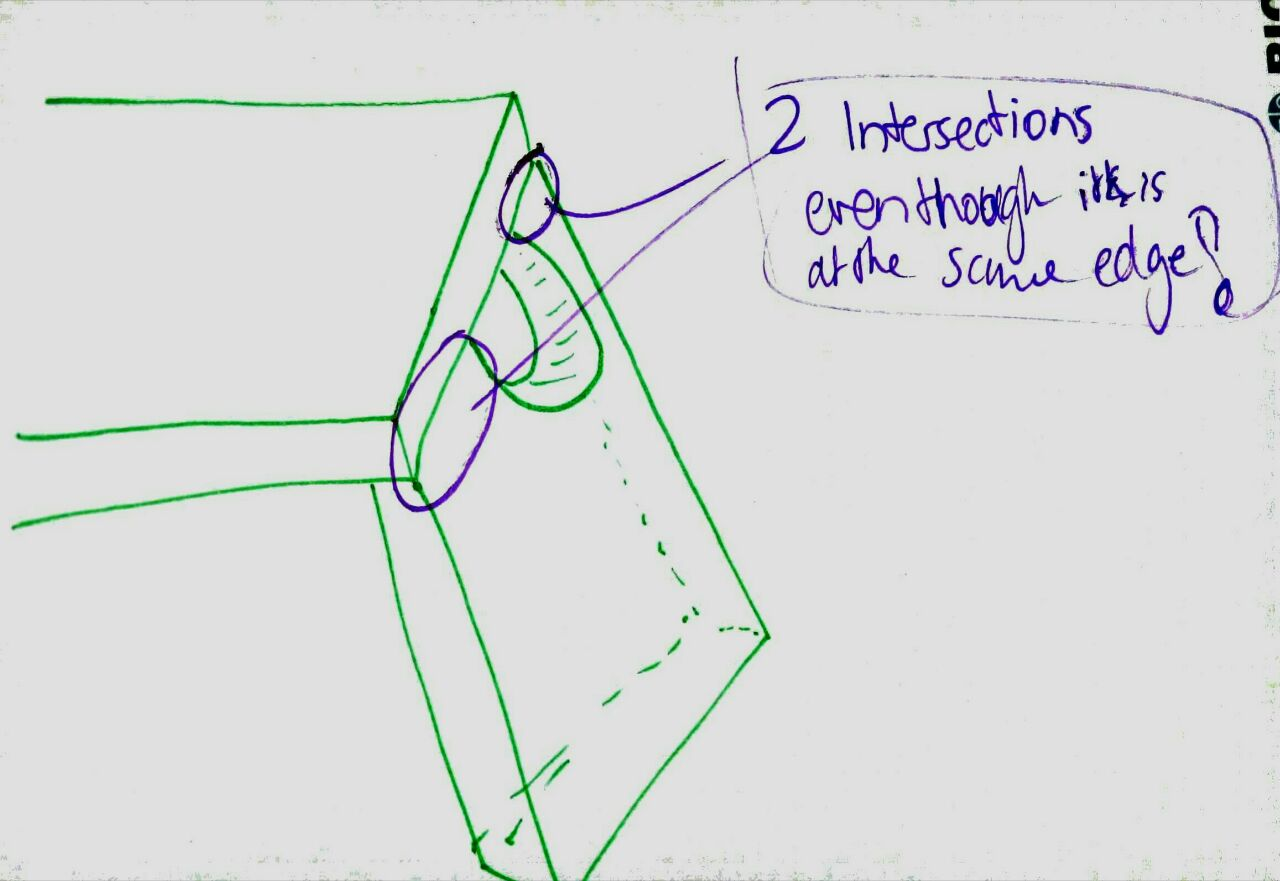
\includegraphics[width=0.5\columnwidth]{Images/06-2-joints-moreThanOneLinePerEdge.jpg}
    \item find out if model is assemblable in the end\\
    A very important information about the final converted model is if it can actually be build. A user may not only need assembly instructions on how to actually build the model when cut but also if it is possible to do so. There may be a conflict when plate a needs to be put up before plate b but plate b also needs to be in the model before plate a. This should not happen or at least be mentioned to the user.
    \item rejoining broken up plates (t-connection)\\
    This is what dustin also suggested and already implemented.\\
    He suggested to group two plates together again when:\\
    \begin{enumerate}
        \item the main sides of P1 and P2 are coplanar
        \item P1 and p2 have the same thickness
        \item P1 and P2 each have a shared edge with p3 that is parallel and which overlaps when projected onto each other
    \end{enumerate}
    It can happen that during finding inherent plates some plates are broken by another. This should result in a t-junction. For this the plategraph has to recognize those broken-up plates and reunion them. \\
    For this the following steps are necessary:
    \begin{enumerate}
        \item Iterate over all nodes and check if it has two or more neighbors. 
        \item Test if the any of the neigbors are coplanar to each other. If so they are labeled as plates p1 and p2. Any other neighbor is labeled p3 or higher.
        \item Check if p1 and p2 have the same thickness. If not start over with the next node
        \item If they have the same thickness the intersections needs to be checked for parallelness and overlaps between p1 and p3 and p2 and p3.
        \item When determined that p1 and p2 are actually one plate which is parted by p3 then they need to be unioned and marked for a t-junction to be handled in the next step.
    \end{enumerate}
    (not sure if this is all it takes maybe a plate is broken up more than once, meaning not only p1 and p2 might be coplanar)
\end{itemize}





% Dummy algorithm:\\
% \begin{algorithm}[H]
% 	\DontPrintSemicolon
% 	\KwData{input Data}
% 	\KwResult{result Data}
% 	initialize variables here\;
%    \caption{Name of Algorithm}

% \end{algorithm}



% \begin{algorithm}[H]
% \DontPrintSemicolon
% 	\KwData{this text}
% 	\KwResult{how to write algorithm with \LaTeX2e }
% 	initialization\;
% 	\While{not at end of this document}{
% 	read current\;
% 	\eIf{understand}{
% 	go to next section\;
% 	current section becomes this one\;
% 	}{
% 	go back to the beginning of current section\;
% 	}
%      \For{all I know}{
%      look at this link to learn more about \LaTeX2e:\;
%      http://ctan.space-pro.be/tex-archive/macros/latex/contrib/algorithm2e/doc/algorithm2e.pdf\;
%      }
% 	}
%    \caption{How to write algorithms}

% \end{algorithm}






\end{document}